\chapter{Results} % Main chapter title







  





  

  
  \label{sec:implementation}
  
  \section{Implementation Details}
  \subsection{Model Details}
  With the Tiny backbone, SiamABC consists of 2.03M parameters and uses 0.628 GigaFLOPs. We refer to this tracker as SiamABC-Tiny or S-Tiny. With the Small backbone, SiamABC consists of 9.82M parameters and uses 6.81 GigaFLOPs. We refer to it as SiamABC-Small or S-Small. S-Tiny runs at 100 FPS on a CPU, 425 FPS on a GPU, and 40 FPS on our edge device Jetson Orin Nano, while S-Small runs at 45 FPS (CPU), 400 FPS (GPU), and 30 FPS (Nano). 
  
  
  \subsection{Training}
  \begin{algorithm}
	\centering
	\caption{Sampling Strategy}\label{alg:sampling}
	\begin{algorithmic}
	\State $X \gets rand(X^n) | X \in X^n$ \Comment{sequence}
	\State $I_T \gets x_i |  x_i \in X$ \Comment{static template}
	\State $I_t \gets x_j | x_j \in X[i, i+\Delta]$ \Comment{search-region} 
	\State $I_S \gets x_k, x_k \in X[i, j]$ \Comment{dynamic-search-region}
	\State $I_D \gets crop(I_S)$ \Comment{dynamic template}
	\end{algorithmic}
  \end{algorithm}
  All the code is written in PyTorch \cite{paszke2019pytorch}. Both models were trained on a single Nvidia RTX A6000 GPU for 20 epochs. We use a batch size of 32 and ADAM optimizer \cite{kingma2014adam} with a learning rate of $10^{-4}$. We sample a random sequence from a database as shown in Algorithm \ref{alg:sampling}. We choose a random frame for the template, $I_T$. Then, we choose another frame randomly for the search-region, $I_t$, from an interval of size $\Delta=150$ right after the frame that contains the template. The dynamic-search-region $I_S$, and $I_D$, are randomly sampled from the interval with the lower bound of the template frame and the upper bound of the search-region frame. Here, we should note that $I_S$ contains $I_D$. We randomly choose 300,000 samples from GOT-10k \cite{Huang2021}, 100,000 from LaSOT \cite{fan2021lasot}, 200,000 from COCO2017 \cite{lin2014microsoft}, and 400,000 from TrackingNet \cite{muller2018trackingnet} datasets to collect a total of $10^6$ samples every epoch. The input size of the template is $128\times128$, and $256\times256$ for the search frames. For standard augmentations, we crop a template with a size increase offset of 0.2 and a search region with an offset of 2.0. We also apply to the search region crops a random scale and shift factor by uniformly drawing samples from (0.65, 1.35) and (0.92,1.08), respectively. We also apply the color augmentation and use the same post-processing as in~\cite{bertinetto2016fully}.
  

  

  \subsection{Inference}
  We evaluate all the trackers on two hardware platforms. One is based on an Nvidia RTX 3090 GPU and 12th Gen Intel i9-12900F CPU. The other is an entry-level GPU-based edge device, Nvidia Jetson Orin Nano, which here we abbreviate to `Nano'. All the FPS numbers were reproduced using these two platforms. 
  
  \section{Comparison with other Trackers} \label{sec:benchmarks}
  We evaluate our SiamABC trackers on 11 challenging benchmarks: AVisT\cite{noman2022avist}, VOT2020\cite{kristan2020eighth}, LaSOT\cite{fan2021lasot}, TrackingNet\cite{muller2018trackingnet}, GOT-10k\cite{Huang2021}, OTB-2015\cite{7001050}, TC128\cite{liang2015encoding}, UAV123\cite{mueller2016benchmark}, NFS30\cite{kiani2017need}, ITB\cite{li2021informative}, and DTB70\cite{drone-tracking}. The FPS numbers were reproduced using the codebase provided by LightTrack \cite{yan2021lighttrack}. We follow GOT-10k\cite{Huang2021} guidelines and use their toolkit \cite{githubGitHubGot10ktoolkit} to evaluate the generic benchmarks. For VOT2020 \cite{kristan2020eighth}, we use their provided toolkit for the challenge. For GOT-10k\cite{Huang2021} and TrackingNet \cite{muller2018trackingnet}, we send the raw results to their servers for a fair evaluation. 
  
  \begin{table}
	\caption{Comparative Study with other SOTA approaches on various benchmarks including AVisT\cite{noman2022avist}, NFS30\cite{kiani2017need}, and UAV123\cite{mueller2016benchmark}. Red, blue, and green colors describe the best three CPU real-time trackers whereas bold suggests the best CPU non-real-time tracker.
	}
	\label{tab:main_res_avist_nfs_uav}
	\centering
	\scalebox{0.8}{
	  \setlength{\tabcolsep}{0.45em}
	\begin{tabular}{c |c c  c  |c c  |c c |c c c}
	
	\hline
	\multirow{3}{*}{Methods} & \multicolumn{7}{c|}{Out-of-Distribution (OOD) test sets} & & \\
	 & \multicolumn{3}{c|}{AVisT\cite{noman2022avist}} & \multicolumn{2}{c|}{NFS30\cite{kiani2017need}} & \multicolumn{2}{c|}{UAV123\cite{mueller2016benchmark}}  & \multicolumn{3}{c}{ FPS ($\uparrow$)}  \\
	 & AUC & OP50 & OP75    & AUC & Prec. & AUC & Prec. & CPU & GPU & Nano\\
	 
	\hline
	\multicolumn{11}{c}{CPU non-real-time Methods} \\
	\hline
  
	STARK-ST50 \cite{yan2021learning}         & 0.511 & 0.592 & \bf{0.391}       & 0.652  & - & 0.691  & - & \bf{7} & 66 & 10\\
	Ocean \cite{zhang2020ocean}               & 0.389 & 0.436 & 0.205       & 0.573  & 0.706 & 0.574  & - & 2  & 70 & 18\\
	SiamRPN++ \cite{li2019siamrpn++}          & 0.390 & 0.435 & 0.212       & 0.596  & \bf{0.720} & 0.593  & - & 1.4 & 145 & 10 \\
	SiamMask \cite{wang2019fast}              & 0.358 & 0.401 & 0.185       & - & -  & - & -  & 4 & \bf{308} & 20 \\
	SiamBAN \cite{chen2020siamese}            & 0.376 & 0.432 & 0.217       & 0.594  & - & 0.631  & 0.833  & 4 & 300 & \bf{24} \\
	SeqTrack-L384 \cite{chen2023seqtrack}     & - & - & -                   & 0.662  & - & 0.685  & - & 0.4 & 15 & -\\
	MixFormerV2-B \cite{cui2024mixformerv2}   & - & - & -                   & -  & - & \bf{0.699}  & \bf{0.921}  & \bf{7} & 130 & 15 \\
	DropMAE \cite{wu2023dropmae}              & - & - & -                   & -  & - & -  & - & 4 & 98 & 10 \\
	TransT \cite{chen2021transformer}         & 0.490 & 0.564 & 0.372       & 0.657  & - & 0.691  & - & \bf{7} & 85 & 8 \\
	OSTrack-256 \cite{ye2022joint}            & - & - & -                   & 0.647  & - & 0.683  & - & 4 & 98 & 18 \\
	ToMP-50 \cite{mayer2022transforming}      & \bf{0.516} & \bf{0.595} & 0.389      & \bf{0.669}  & - & 0.690  & - & \bf{7} & 83 & 6 \\
	
	\hline
	\multicolumn{11}{c}{CPU real-time Methods} \\
	\hline  
	
	HiT-Small~\cite{kang2023exploring} & - & - & - &  0.618 & - & 0.633 & - & - & - & -\\
	SMAT \cite{gopal2024separable} & \color{ForestGreen} \bf{0.447} & \color{ForestGreen} \bf{0.507} & \color{ForestGreen} \bf{0.313}  &  \color{RoyalBlue} \bf{0.620}  &  \color{RoyalBlue} \bf{0.746} & \color{ForestGreen} \bf{0.643}  & \color{ForestGreen} \bf{0.839} & 34 & 158 & 20 \\
	E.T.Track \cite{blatter2023efficient} & 0.390 & 0.412 & 0.227               & 0.570  & 0.694 & 0.623  & 0.806 & 35 & 108 & 10 \\
	MixFormerV2-S \cite{cui2024mixformerv2} & 0.396 & 0.425 & 0.227             & 0.610  & 0.722 & 0.634  & 0.837 & 37 & \color{ForestGreen} \bf{420} & \color{Mahogany} \bf{40} \\
	HCAT \cite{chen2022efficient} & 0.418 & 0.481 & 0.263                       & \color{ForestGreen} \bf{0.619}  & 0.741 & 0.636  & 0.805 & \color{ForestGreen} \bf{60} & 300 & \color{ForestGreen} \bf{24} \\
	LightTrack \cite{yan2021lighttrack} & 0.404 & 0.437 & 0.242                 & 0.565  & 0.692 & 0.617  & 0.799 & \color{RoyalBlue} \bf{67} & 170 & 17 \\
	FEAR-XS \cite{borsuk2022fear} & 0.387 & 0.421 & 0.220                       & 0.486  & 0.563 & 0.610  & 0.816 &  \color{Mahogany} \bf{100} & \color{Mahogany} \bf{450} & \color{Mahogany} \bf{40}\\
  
	
	\rowcolor{lightgray!20} \bf{S-Tiny}  &  \color{RoyalBlue} \bf{0.472} &  \color{RoyalBlue} \bf{0.543} &  \color{RoyalBlue} \bf{0.353}  &  \color{RoyalBlue} \bf{0.620}  &  \color{Mahogany} \bf{0.747} &  \color{RoyalBlue} \bf{0.662} &  \color{RoyalBlue} \bf{0.856} &  \color{Mahogany} \bf{100} & \color{RoyalBlue} \bf{425} & \color{Mahogany} \bf{40}\\
	\rowcolor{lightgray!20} \bf{S-Small} &  \color{Mahogany} \bf{0.479} &  \color{Mahogany} \bf{0.557} &  \color{Mahogany} \bf{0.372}  &  \color{Mahogany} \bf{0.624}  & \color{ForestGreen} \bf{0.744} &  \color{Mahogany} \bf{0.681}  &  \color{Mahogany} \bf{0.858} &  45 & 400 & \color{RoyalBlue} \bf{30}\\
	\hline
	\end{tabular}
	}
  \end{table}

  \subsection{AVisT} 
  AVisT~\cite{noman2022avist} consists of 120 extremely challenging real-world sequences in adverse visibility.
  In addition to simple occlusion and fast motion, it involves objects under heavy rain, heavy snow, dense fog, sandstorms, hurricanes, etc. In \ref{tab:main_res_avist_nfs_uav}, we note that this out-of-distribution benchmark highlights a significant performance degradation of SOTA trackers compared to the widely used in-distribution test sets. On the other hand, our trackers, S-Tiny and S-Small, are outperforming HCAT by 5.4\% and 6.1\% respectively and MixFormerV2-S\cite{cui2024mixformerv2} by 7.6\% and 8.3\% respectively, showing our approach's improved ability to track in sequences with adverse conditions. Additionally, S-Tiny outperforms SMAT\cite{gopal2024separable} by 2.5\% while being almost 3x faster on a CPU. We show qualitative results on this benchmark, comparing S-Tiny with other trackers in \ref{fig:qual_compare_bbox}. S-Tiny shows remarkable resilience against adverse visibility conditions. 
  
  \subsection{UAV123}
  UAV123~\cite{mueller2016benchmark}  is a benchmark for tracking from an aerial viewpoint involving 123 long video sequences. We outperform HCAT by 2.6\% and 4.5\% respectively, and SMAT by 1.9\% and 3.8\% respectively, confirming the OOD generalization ability of our approach illustrated in \ref{tab:main_res_avist_nfs_uav}.


  \subsection{NFS30}
  NFS30~\cite{kiani2017need}  is a benchmark collected with extremely high frame rate of 240 FPS for fast tracking. Similar to other approaches, we use the 30 FPS version of the benchmark for evaluation. Our trackers outperform others also in this OOD test. Please refer to \ref{tab:main_res_avist_nfs_uav}.
  
  \subsection{VOT2020}  
  \begin{table}
	\caption{Comparative study on VOT2020 Benchmark \cite{kristan2020eighth}. Red, blue, and green colors describe the best three CPU real-time trackers whereas bold suggests the best CPU non-real-time tracker.}
	
	\label{tab:vot2020_res}
	\centering
	\scalebox{0.8}{
	
	\begin{tabular}{c| c c c| c c c}
	\hline
	\multirow{2}{*}{Trackers} 	& \multicolumn{3}{c|}{VOT2020~\cite{kristan2020eighth}} & \multicolumn{3}{c}{ FPS ($\uparrow$)}  \\
								& EAO & Accuracy & Robustness & CPU & GPU & Nano \\
	\hline
	\multicolumn{7}{c}{CPU non-real-time Methods} \\
	\hline
	STARK-ST50 \cite{yan2021learning} 			& \bf{0.308} & \bf{0.478} & \bf{0.799}  & 6 & 66 & 10 \\
	STARK-S50 \cite{yan2021learning} 			& 0.280 & 0.477 & 0.728  & 7 & 66 & \bf{12} \\
	DiMP \cite{bhat2019learning} 				& 0.274 & 0.457 & 0.740  & \bf{14} & \bf{127} & 10 \\
	\hline
	\multicolumn{7}{c}{CPU real-time Methods} \\
	\hline
	HCAT \cite{chen2022efficient}  				& \color{RoyalBlue} \bf{0.276} & \color{ForestGreen} \bf{0.455} &  \color{Mahogany} \bf{0.747} & \color{ForestGreen} \bf{60} & \color{ForestGreen} \bf{300}  & \color{RoyalBlue} \bf{24}  \\
	E.T.Track \cite{blatter2023efficient} 		& 0.267 & 0.432  &  \color{RoyalBlue} \bf{0.741} & 35 & 108 & 10 \\
	LightTrack \cite{yan2021lighttrack}  		& 0.242 & 0.422 & 0.689 & \color{RoyalBlue} \bf{67} & 170 & \color{ForestGreen} \bf{17} \\
	ATOM \cite{danelljan2019atom}				& \color{ForestGreen} \bf{0.271} & \color{RoyalBlue} \bf{0.462} & \color{ForestGreen} \bf{0.734} & 30 & 240 & 13 \\
	MixFormerV2-S \cite{cui2024mixformerv2} 	& 0.258 & - & - & 37 & \color{RoyalBlue} \bf{420} & \color{Mahogany} \bf{40} \\

	\rowcolor{lightgray!20} \bf{S-Tiny}   		& \color{Mahogany} \bf{0.291} & \color{Mahogany} \bf{0.491} & \color{RoyalBlue} \bf{0.741} & \color{Mahogany} \bf{100} & \color{Mahogany} \bf{425} & \color{Mahogany} \bf{40} \\
	\hline
	\end{tabular}
	}
	\end{table}
  VOT2020~\cite{kristan2020eighth} contains 60 challenging videos and employs EAO (expected average overlap) as its metric alongside the accuracy and robustness. In \ref{tab:vot2020_res}, our tracker, S-Tiny, shows remarkable resilience against difficult scenarios in this benchmark, outperforming HCAT\cite{chen2022efficient} (best real-time method) and STARK-S50\cite{yan2021learning} by 1.05\% and 1.04\% EAO respectively while being more than 14x faster than STARK-S50 on a CPU.

  \begin{table}
	\caption{Comparative Study with other SOTA approaches on various benchmarks including TrackingNet\cite{muller2018trackingnet}, GOT-10k\cite{Huang2021}, and LaSOT\cite{fan2021lasot}. Red, blue, and green colors describe the best three CPU real-time trackers whereas bold suggests the best CPU non-real-time tracker.
	}
	\label{tab:main_res_tn_lasot_got}
	\centering
	\scalebox{0.8}{
	  \setlength{\tabcolsep}{0.45em}
	\begin{tabular}{c |c c  c |c c |c c |c c c}
	
	\hline
	\multirow{3}{*}{Methods}  & \multicolumn{7}{c|}{In-Distribution (ID) test sets} & & \\
	 & \multicolumn{3}{c|}{TrackingNet\cite{muller2018trackingnet}} & \multicolumn{2}{c|}{GOT-10k\cite{Huang2021}} & \multicolumn{2}{c|}{LaSOT\cite{fan2021lasot}}  & \multicolumn{3}{c}{ FPS ($\uparrow$)}  \\
	 & AUC & P$_{norm}$ & Prec. & AO & SR$_{0.50}$ & AUC & Prec. & CPU & GPU & Nano\\
	 
	\hline
	\multicolumn{11}{c}{CPU non-real-time Methods} \\
	\hline
  
	STARK-ST50 \cite{yan2021learning}         & 0.813  & 0.861  & - & 0.680  & 0.777 & 0.666  & -  & \bf{7} & 66 & 10\\
	Ocean \cite{zhang2020ocean}               & -  & -  & - & 0.611  & 0.634  & 0.505  & 0.517 & 2  & 70 & 18\\
	SiamRPN++ \cite{li2019siamrpn++}          & 0.733  & 0.800  & - & -  &  - & 0.503  & 0.496  & 1.4 & 145 & 10 \\
	SiamMask \cite{wang2019fast}              & -  & - & -  & -  & - & - & -  & 4 & \bf{308} & 20 \\
	SiamBAN \cite{chen2020siamese}            & -  & -  & - & -  & - & 0.514  & 0.598 & 4 & 300 & \bf{24} \\
	SeqTrack-L384 \cite{chen2023seqtrack}     & \bf{0.855}  & \bf{0.895}  & \bf{0.858} & 0.748  & 0.819  & \bf{0.725}  & 0.793  & 0.4 & 15 & -\\
	MixFormerV2-B \cite{cui2024mixformerv2}   & 0.834  & 0.881  & 0.816 & 0.739  & -  & 0.706  & \bf{0.808}  & \bf{7} & 130 & 15 \\
	DropMAE \cite{wu2023dropmae}              & 0.841  & 0.889  & - & \bf{0.759}  & \bf{0.868}  & 0.718  & 0.780  & 4 & 98 & 10 \\
	TransT \cite{chen2021transformer}         & 0.814  & 0.867  & 0.803 & 0.723  & 0.824   & 0.649  & 0.690  & \bf{7} & 85 & 8 \\
	OSTrack-256 \cite{ye2022joint}            & 0.831  & 0.878  & 0.820 & 0.710  & 0.804  & 0.691  & 0.752 & 4 & 98 & 18 \\
	ToMP-50 \cite{mayer2022transforming}      & 0.786  & 0.862  & 0.812 & -  & - & 0.676  & 0.722  & \bf{7} & 83 & 6 \\
	
	\hline
	\multicolumn{11}{c}{CPU real-time Methods} \\
	\hline  
	
	HiT-Small~\cite{kang2023exploring} & \color{ForestGreen} \bf{0.777} & 0.819 & \color{ForestGreen} \bf{0.731} & 0.626 & 0.712 & 0.605 & \color{ForestGreen} \bf{0.615} & - & - & -\\
	SMAT \cite{gopal2024separable} &  \color{Mahogany} \bf{0.786} &  \color{Mahogany} \bf{0.842}  &  \color{Mahogany} \bf{0.756} &  \color{RoyalBlue} \bf{0.645}  &  \color{RoyalBlue} \bf{0.747} &  \color{Mahogany} \bf{0.617}  &  \color{Mahogany} \bf{0.646}  & 34 & 158 & 20 \\
	E.T.Track \cite{blatter2023efficient} & 0.745  & 0.798  & 0.698 & 0.566  & 0.646 & 0.589  & 0.603 & 35 & 108 & 10 \\
	MixFormerV2-S \cite{cui2024mixformerv2} & 0.758  & 0.811  & 0.704 & 0.587  & 0.672 & \color{ForestGreen} \bf{0.606}  & 0.604  & 37 & \color{ForestGreen} \bf{420} & \color{Mahogany} \bf{40} \\
	HCAT \cite{chen2022efficient} & 0.766  & \color{ForestGreen} \bf{0.826}  & 0.729 & \color{ForestGreen} \bf{0.634}  & \color{ForestGreen} \bf{0.743} & 0.590  & 0.605 & \color{ForestGreen} \bf{60} & 300 & \color{ForestGreen} \bf{24} \\
	LightTrack \cite{yan2021lighttrack} & 0.729  & 0.793  & 0.699 & 0.582  & 0.660  & 0.522  & 0.517 & \color{RoyalBlue} \bf{67} & 170 & 17 \\
	FEAR-XS \cite{borsuk2022fear} & 0.387 & 0.805 & 0.699 & 0.573  & 0.681  & 0.535  & 0.545 &  \color{Mahogany} \bf{100} & \color{Mahogany} \bf{450} & \color{Mahogany} \bf{40}\\
  
	
	\rowcolor{lightgray!20} \bf{S-Tiny}  & 0.741  & 0.819  & 0.720 & 0.614  & 0.728 & 0.590  &  0.607  &  \color{Mahogany} \bf{100} & \color{RoyalBlue} \bf{425} & \color{Mahogany} \bf{40}\\
	\rowcolor{lightgray!20} \bf{S-Small} & \color{RoyalBlue} \bf{0.784}  & \color{RoyalBlue} \bf{0.835}  & \color{RoyalBlue} \bf{0.746} & \color{Mahogany} \bf{0.646}  &  \color{Mahogany} \bf{0.751}  & \color{RoyalBlue} \bf{0.607}  & \color{RoyalBlue} \bf{0.622}  &  45 & 400 & \color{RoyalBlue} \bf{30}\\
	\hline
	\end{tabular}
	}
  \end{table}

  \subsection{LaSOT, TrackingNet, and GOT-10k}
  
  The LaSOT~\cite{fan2021lasot} benchmark involves 280 long test sequences with 2500 frames per sequence on average.
  GOT-10k~\cite{Huang2021} is a challenging short term benchmark consisting of 180 test sequences which are evaluated on their server. Most approaches are trained on the large training sets of LaSOT, TrackingNet, and GOT-10k; thus, the test distributions of such benchmarks remain quite similar. 
  Nevertheless, S-Small outperforms most SOTA CPU real-time trackers in these benchmarks while remaining efficient as shown in \ref{tab:main_res_tn_lasot_got}. Our approach slightly underperforms SMAT
  in two ID sets, LaSOT and TrackingNet; however, we note that the trade-off with speed is significant as SMAT runs at 34 FPS (CPU), 158 FPS (GPU), and 20 FPS (Nano), while S-tiny runs at 100 FPS (CPU), 425 FPS (GPU), and 40 FPS (Nano), and S-Small runs at 45 FPS (CPU), 400 FPS (GPU), and 30 FPS (Nano). 
  
  \begin{table}
	\caption{Comparative study on ITB \cite{li2021informative}, OTB \cite{7001050}, TC128 \cite{liang2015encoding}, and  DTB70 \cite{drone-tracking} benchmarks in terms of their AUC score. Red, blue, and green colors describe the best three CPU real-time trackers whereas bold suggests the best CPU non-real-time tracker.}
	\label{tab:itb_otb_tc_dtb_res}
	\centering
	\scalebox{0.8}{
	
	\begin{tabular}{c| c | c | c | c| c c c}
	\hline
	\multirow{2}{*}{Trackers} 	& \multicolumn{4}{c|}{Benchmarks} & \multicolumn{3}{c}{ FPS ($\uparrow$)}  \\
								& ITB \cite{li2021informative} & OTB \cite{7001050} &  TC128 \cite{liang2015encoding} & DTB70 \cite{drone-tracking} & CPU & GPU & Nano \\
	\hline
	\multicolumn{8}{c}{CPU non-real-time Methods} \\
	\hline
	DropMAE \cite{wu2023dropmae} 					& \bf{0.650} & \bf{0.696} & - & - & 4 & 85 & 10 \\
	TransT  \cite{chen2021transformer} 				& 0.547 & 0.695  & 0.596 & \bf{0.667} & 8 & 66 & 8 \\
	STARK \cite{yan2021learning} 					& 0.576 & 0.681 & \bf{0.626} & 0.638 & 7 & 66 & 12 \\
	DiMP \cite{bhat2019learning} 					& 0.537 & 0.684 & 0.612 & - & \bf{14} & 127 & 10 \\
	SiamRPN++ \cite{li2019siamrpn++}				& 0.441 & 0.687 & 0.577 & 0.569 & 1.4 & \bf{145} & 10 \\
	Ocean \cite{zhang2020ocean}						& 0.477 & 0.684  & 0.557 & 0.455 & 2 & 70 & \bf{18} \\
	\hline
	\multicolumn{8}{c}{CPU real-time Methods} \\
	\hline
	E.T.Track \cite{blatter2023efficient} 			& - & \color{ForestGreen} \bf{0.678} & - & - & 35 & 108 & 10 \\
	LightTrack \cite{yan2021lighttrack}  			& - & 0.662 & 0.550 & \color{ForestGreen} \bf{0.491} & \color{RoyalBlue} \bf{67} & 170 & \color{ForestGreen} \bf{17} \\
	ATOM \cite{danelljan2019atom}					& \color{ForestGreen} \bf{0.472} & 0.669 & \color{ForestGreen} \bf{0.599} & - & 30 &  \color{ForestGreen} \bf{240} &  13 \\

	\rowcolor{lightgray!20} \bf{S-Tiny}   			& \color{RoyalBlue} \bf{0.548} & \color{RoyalBlue} \bf{0.709} & \color{RoyalBlue} \bf{0.617} & \color{RoyalBlue} \bf{0.656} & \color{Mahogany} \bf{100} & \color{Mahogany} \bf{425} & \color{Mahogany} \bf{40} \\
	\rowcolor{lightgray!20} \bf{S-Small}   			& \color{Mahogany} \bf{0.555} & \color{Mahogany} \bf{0.713} & \color{Mahogany} \bf{0.630} & \color{Mahogany} \bf{0.662} & \color{ForestGreen} \bf{45} & \color{RoyalBlue} \bf{400} & \color{RoyalBlue} \bf{30} \\
	\hline
	\end{tabular}
	}
	\end{table}

  \subsection{OTB-2015, TC128, DTB70, and ITB}
  As shown in \ref{tab:itb_otb_tc_dtb_res}, we outperform other CPU-based trackers on the \textbf{OTB-2015}\cite{7001050} benchmark with 100 sequences, even surpassing the CPU non-real-time approaches. 
  Another similar benchmark is \textbf{TC128}\cite{liang2015encoding} with 128 challenging color sequences, where we outperform other SOTA approaches as well. \textbf{DTB70}\cite{drone-tracking} is another small-scale UAV benchmark involving 70 long sequences. We consistently show improvement here as well. \textbf{ITB}\cite{li2021informative} is a benchmark with 180 various challenging sequences from many other benchmarks giving an informative evaluation of trackers. ITB is second to AVisT in terms of challenging sequences, and \ref{tab:itb_otb_tc_dtb_res} confirms a remarkable generalization ability of our approach. We note that DropMAE \cite{wu2023dropmae} was pre-tained on additional diverse training data.
  
  
  
  \begin{table}[h]
	\caption{Comparative study on test-time adaptation (TTA) approaches on AVisT\cite{noman2022avist} as it involves various extreme distribution shifts with real-world corruptions and ITB \cite{li2021informative} as the next most challenging benchmark. The best results are in bold.
	}
	\label{tab:tta_res}
	\centering
	\scalebox{0.78}{
	\begin{tabular}{c|c c  c c |c c  c c |c c c}
	
	\hline
	
	\multirow{2}{*}{Methods}  & \multicolumn{4}{c|}{AVisT\cite{noman2022avist}}  & \multicolumn{4}{c|}{ITB\cite{li2021informative}} &  \multicolumn{3}{c}{Latency (ms) $\downarrow$ }  \\
	 & AUC & OP50 & OP75 & Prec.    & AUC & OP50 & OP75 & Prec. & CPU & GPU & Nano\\
  
	\hline 
	No TTA & 0.458 & 0.529 & 0.340 & 0.413 & 0.539 & 0.659 & 0.483 & 0.631 & \bf{3.6} & \bf{0.6} & \bf{9.8}\\
	\hline
	\multicolumn{12}{c}{Backward-Based Methods} \\
	\hline
	TENT \cite{wang2020tent} & 0.460 & 0.518 & 0.356 & 0.417 & 0.530 & 0.635 & 0.472 & 0.610 & 9.9 & 2.9 & 30.4 \\
	ETA \cite{niu2022efficient} & 0.459 & 0.516 & \bf{0.360} & 0.416 & 0.525 & 0.630 & 0.470 & 0.606 & 9.9 & 2.8 & 35.6 \\
	\hline
	\multicolumn{12}{c}{Backward-Free Methods} \\
	\hline
	Momentum \cite{schneider2020improving} & 0.452 & 0.513 & 0.341 & 0.411 & 0.540 & 0.656 & 0.484 & 0.632 & 3.7 & 0.7 & 15.1 \\
	DUA \cite{mirza2022norm} & 0.427 & 0.484 & 0.307 & 0.394 & 0.516 & 0.628 & 0.467 & 0.591 & 3.7 & 0.7 & 15.1 \\
	IN \cite{pan2018two} & 0.454 & 0.515 & 0.342 & 0.417 & 0.519 & 0.628 & 0.455 & 0.604 & 6.6 & 1.9 & 23.1 \\
	AdaBN \cite{li2016revisiting} & 0.456 & 0.517 & 0.345 & 0.414 & 0.522 & 0.632 & 0.461 & 0.608 & 3.7 & 0.7 & 15.1 \\
	\rowcolor{lightgray!20} DTTA (ours) & \bf{0.472} & \bf{0.543} & 0.353 & \bf{0.440} & \bf{0.548} & \bf{0.667} & \bf{0.494} & \bf{0.634} & 3.7 & 0.7 & 15.1 \\
	\hline
	\end{tabular}
	}
  \end{table}
	
  \section{Comparision with Adaptation Approaches}\label{sec:tta_res}
  There are no specific Test-Time Adaptation (TTA) approaches available for single-object tracking. Therefore, to compare our Dynamic TTA strategy mentioned in \ref{sec:methods_tta}, we implement relevant backward-free and backward-based baselines according to the codebase provided by \cite{alfarra2023revisiting}. We carefully follow the instructions provided by the respective approaches and use them under our online setting. 
  In our S-Tiny model we incorporate TENT\cite{wang2020tent} and ETA\cite{niu2022efficient} as our TTA baselines with backward-passes,
  where we use our classification output as self-entropy. Additionally, we also evaluated Momentum\cite{schneider2020improving}, DUA\cite{mirza2022norm}, IN\cite{pan2018two}, and AdaBN\cite{li2016revisiting} as our backward-free TTA baselines. We set the batch size to 1. The comparison is shown in \ref{tab:tta_res} with two of the most challenging benchmarks, AVisT as it involves multiple adverse scenarios with natural corruptions and ITB as the next most challenging benchmark.
  TENT and ETA have almost 3x the latency because of the backward passes, and do improve with AVisT. However, we do not observe the same with ITB. Momentum shows negligible improvement, whereas IN, AdaBN, and DUA show performance degradation in both scenarios. When DTTA, our efficient adaptation strategy, is turned on, we notice significant improvement with both benchmarks while having minimal latency. Essentially, our approach continually adapts to the new domains without forgetting as the BN-statistics stay anchored to the source statistics and model parameters remain frozen. Additionally, our approach continually adapts to each new instance with negligible difference in latency.

  
  \section{Ablation Study}\label{sec:ablation}
  
  
  
  We perform ablation studies on each of the components of S-Tiny used on AVisT as an OOD benchmark and on LaSOT as an ID benchmark. In \ref{fig:all_ablation}(top), the baseline is obtained by removing the FMF block and the TRL losses, $\mathcal{L}_{TR}$ and $\mathcal{L}_{Reg}$. Next, we add the intermediate dynamic frames to obtain the mix configuration, without FMF, and lastly, we add our FMF block. We clearly observe the impact of the FMF block, especially on the OOD benchmark, where the AUC increases from 41.8\% to 43.7\%. We also show qualitative results regarding the FMF layer compared to the baseline and the naive concatenation of features in \ref{fig:qual_compare_bbox_abl}, visually showing the significance of our FMF layer. 
  Next, \ref{fig:all_ablation}(middle) shows the ablation on the TRL losses, $\mathcal{L}_{TR}$ and $\mathcal{L}_{Reg}$. The addition of either of them improves performance; however, the improvement is more significant when used together.
  Further, in \ref{tab:att_comp} we test the impact of FMF on accuracy compared to PSA\cite{liu2021polarized}, observing no noticeable fluctuations in performance.
  We further evaluate the squeeze rate of our FMF block in \ref{fig:all_ablation}(bottom). There we notice performance degradation on the OOD benchmark when we do not squeeze the FMF module, but not as much in the ID benchmark, suggesting that squeeze is more important for accurate filtration of OOD sequences.
  In \ref{tab:component_ablation_updates}, we show a case-study on parameter-free dynamic update strategies, where ours consistently improves over the others.
  
  \begin{figure}
	\centering
	 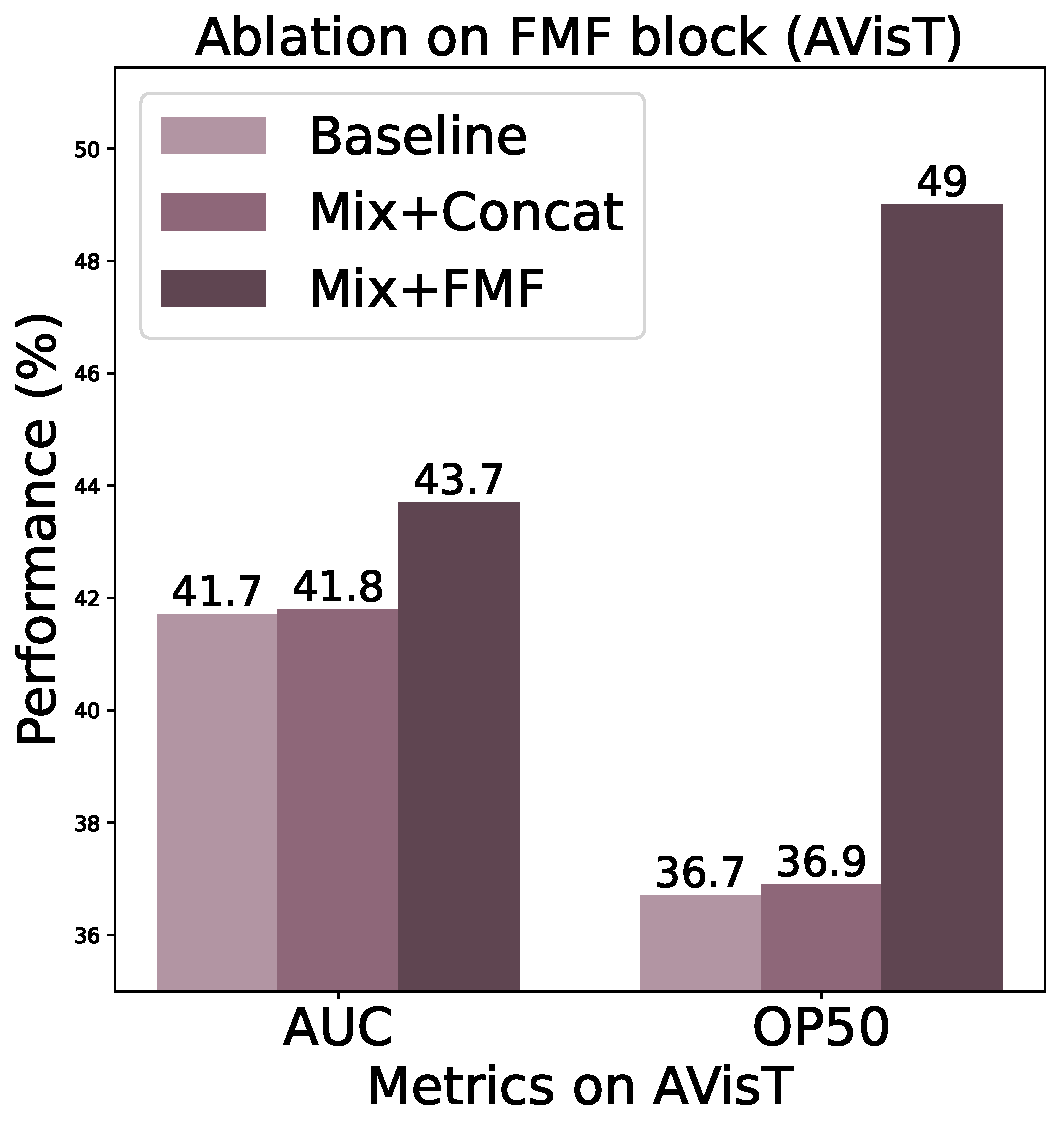
\includegraphics[width=6cm]{figures/abl_fmf_avist.pdf}
	 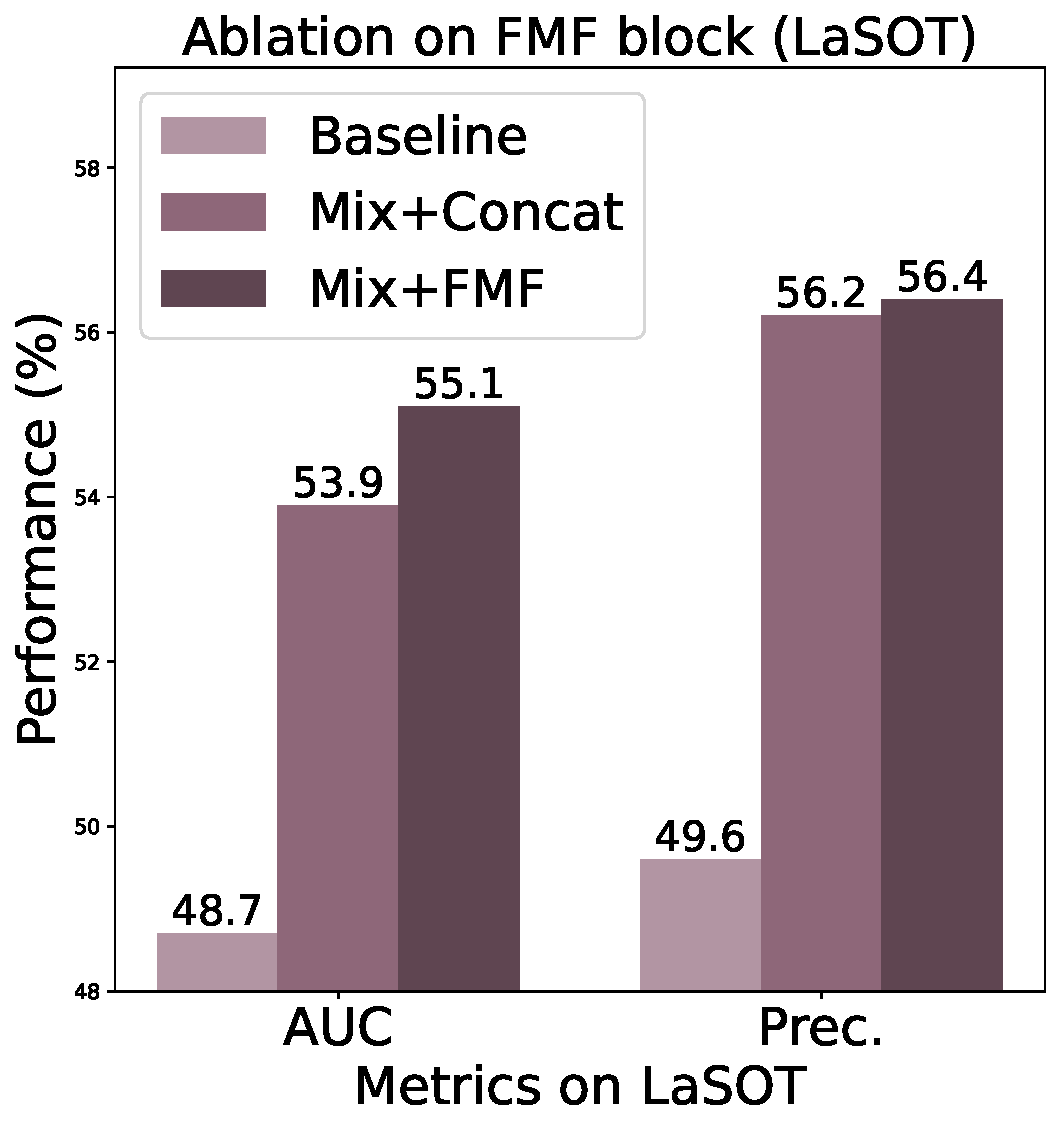
\includegraphics[width=6cm]{figures/abl_fmf_lasot.pdf}
	 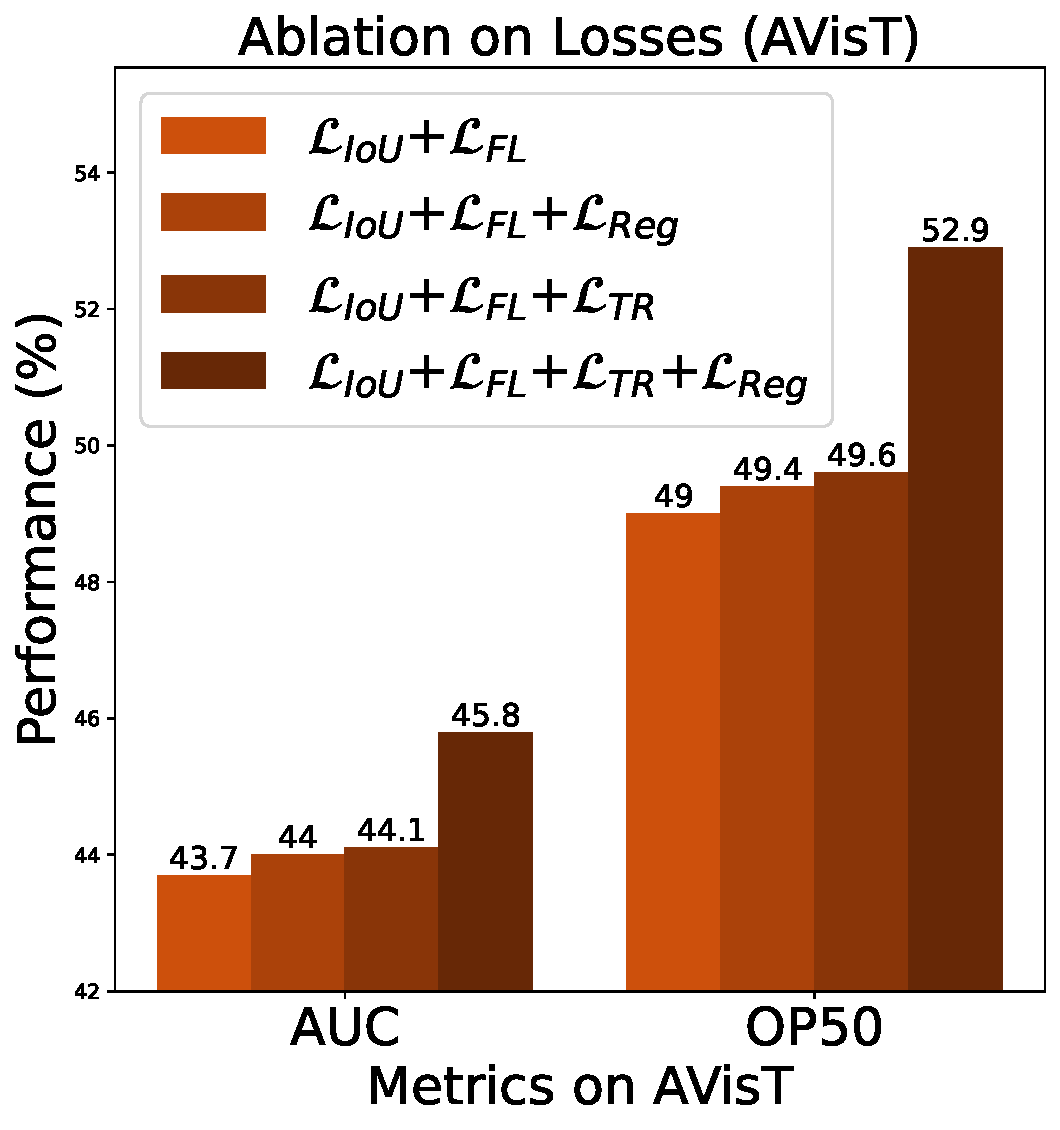
\includegraphics[width=6cm]{figures/abl_losses_avist.pdf}
	 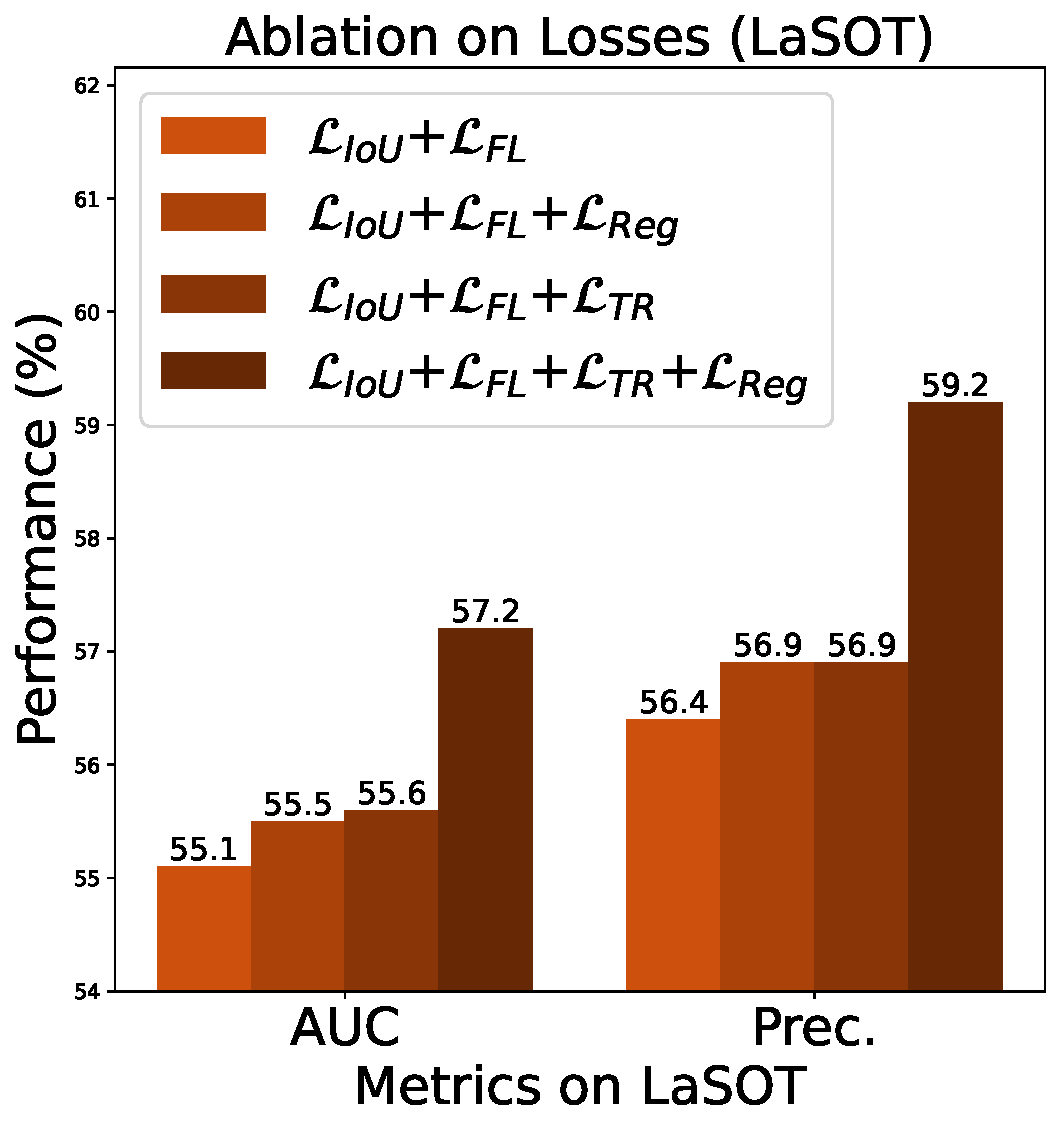
\includegraphics[width=6cm]{figures/abl_losses_lasot.pdf}
	 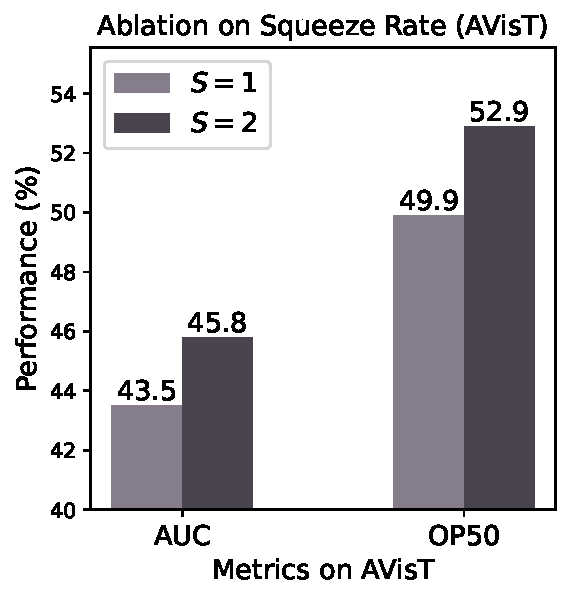
\includegraphics[width=6cm]{figures/abl_sr_avist.pdf}
	 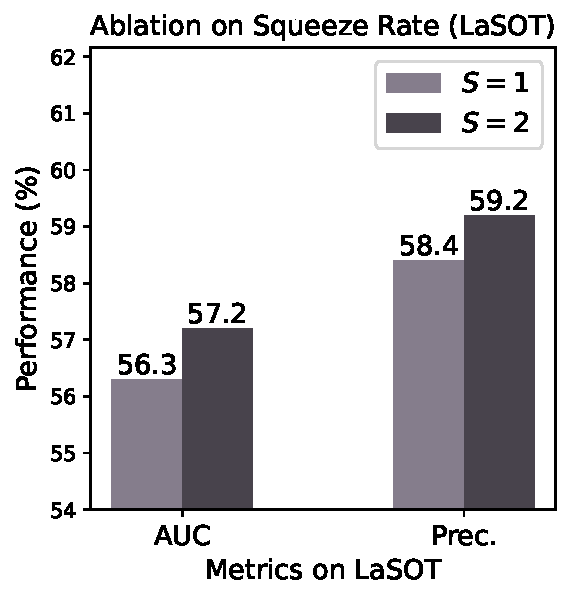
\includegraphics[width=6cm]{figures/abl_sr_lasot.pdf}
	 \vspace{-4mm}
	 \caption{Ablation study on the components of SiamABC-Tiny. Top-row: Ablation on the FMF block. Middle-row: Ablation on TRL losses. Bottom-row: Ablation on squeeze rate.}
	 \label{fig:all_ablation}
	 \vspace{-5mm}
   \end{figure}


   \begin{table}
	\caption{Case study on parameter-free dynamic updates. }
	\label{tab:component_ablation_updates}
	\centering
	\scalebox{0.8}{
	\begin{tabular}{c|c c | c c | c c c}
	\hline
	\multirow{2}{*}{{\shortstack{ Dynamic Updates \\ (No DTTA)} } }  & \multicolumn{2}{c|}{AVisT}   & \multicolumn{2}{c|}{LaSOT} & \multicolumn{3}{c}{FPS($\uparrow$)} \\
	  & AUC & OP50 & AUC & Prec.  & CPU & GPU & Nano \\
	
	\hline
	No Updates & 0.448 & 0.511  & 0.556 & 0.572 & 102 & 430 & 40 \\
	Fixed interval ($N=60$) & 0.445 & 0.514  & 0.519 & 0.533 & 100 & 425 & 40 \\
	FEAR-based \cite{borsuk2022fear} & 0.454 & 0.517  & 0.524 & 0.234 & 96 & 405 & 38 \\
	TATrack-based \cite{he2023target} & 0.361 & 0.377  & 0.414 & 0.430 & 60 & 250 & 22 \\
	\rowcolor{lightgray!20} Ours  & 0.458 & 0.529 & 0.572 & 0.592 & 100 & 425 & 40\\
	\hline
	\end{tabular}
	}
  \end{table}



\begin{figure}
  \hspace*{-35pt}
    \centering
     \includegraphics[width=18cm]{figures/qaual_compare_bbox.pdf}
     \caption{Qualitative comparison on the AVisT \cite{noman2022avist} dataset with other efficient trackers, and with the further inclusion of Ocean. Under adverse visibility conditions, our tracker, S-Tiny, is relatively stable compared to the others while running at 100 FPS on a CPU.}
     \label{fig:qual_compare_bbox}
\end{figure}

\begin{figure}
	\hspace*{-35pt}
    \centering
     \includegraphics[width=18cm]{figures/qaual_compare_bbox_abl.pdf}
     \caption{ Qualitative results on the ablation study of the FMF layer on the AVisT \cite{noman2022avist} dataset. We notice the higher stability of our tracker when using FMF in terms of overalps with the ground truth (green), in comparison to the baseline and the naive concatenation.}
     \label{fig:qual_compare_bbox_abl}
\end{figure}
  %%% Local Variables:
  %%% mode: latex
  %%% TeX-master: "../main"
  %%% End:
  